\begin{dang}{Bài toán vận dụng khái niệm thể tích.}
	Dựa vào khái niệm thể tích để tính chiều cao, khoảng cách, diện tích đa giác, tỉ số thể tích.
	\begin{itemize}
		\item Thể tích khối chóp có diện tích đáy là $S$ và chiều cao $h$ là $V=\dfrac{1}{3}S\cdot h$.
		\item Thể tích khối chóp cụt có diện tích hai đáy lần lượt là $S$ và $S'$, chiều cao $h$ là $$V=\dfrac{1}{3}\cdot\left(S+S'+\sqrt{S\cdot S'}\right)\cdot h.$$
		\item Thể tích khối lăng trụ có diện tích đáy là $S$ và chiều cao $h$ là $V=S\cdot h$. 
	\end{itemize}
\end{dang}
\subsubsection{Ví dụ minh hoạ}
\begin{vd}%[DCHT Toán 11 - KNTT -Vũ Hồng Toàn]%[1K7YQ-3]
	Cho khối chóp và khối lăng trụ có cùng chiều cao và diện tích đáy. Gọi $V$ là thể tích khối lăng trụ và $V_1$ là thể tích khối chóp. Tính tỉ số $\dfrac{V_1}{V}$.
	\dapso{$\dfrac{V_1}{V}=\dfrac{1}{3}$.}
	\loigiai{
		Gọi $S$ là diện tích đáy và $h$ là chiều cao tương ứng của khối lăng trụ và khối chóp.\\
		Ta có
		$$\dfrac{V_1}{V}=\dfrac{\dfrac{1}{3}S\cdot h}{S\cdot h}=\dfrac{1}{3}.$$
	}
\end{vd}
\begin{vd}%[DCHT Toán 11 - KNTT -Vũ Hồng Toàn]%[1K7YQ-3]
	Cho hình lăng trụ tứ giác đều có cạnh đáy bằng $a$ và thể tích $V=2a^3$. Tính chiều cao $h$ của khối lăng trụ đó.
	\dapso{$h=2a$.}
	\loigiai{
		Từ giả thiết, ta có $S=a^2$. Khi đó
		$$V=S\cdot h\Rightarrow h=\dfrac{V}{S} =\dfrac{2a^3}{a^2}=2a.$$
	}
\end{vd}

\begin{vd}%[DCHT Toán 11 - KNTT -Vũ Hồng Toàn]%[1K7BQ-3]
	\immini{
		Cho hình hộp chữ nhật $ABCD.A'B'C'D'$ có $AB=2a$, $AD=a$ và thể tích $V=8a^3$. Tính khoảng cách giữa hai đường thẳng $BC$ và $B'D'$.	
	}
	{
		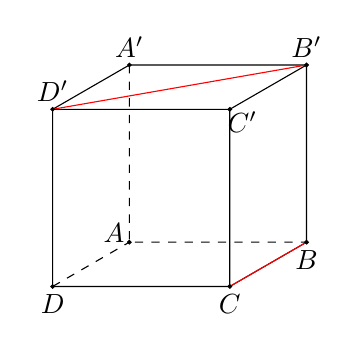
\begin{tikzpicture}[scale=.75]
			\def\a{3}
			\path 
			(0:0) coordinate (A) 
			(0:\a) coordinate (B)++(-150:\a/2) coordinate (C) ++ (180:\a) coordinate (D)
			(90:\a) coordinate (A')++(0:\a) coordinate (B')++(-150:\a/2) coordinate (C') ++ (180:\a) coordinate (D')
			;
			\draw[dashed] (A')--(A)--(B) (D)--(A);
			\draw (D')--(A')--(B')--(C') (B)--(B') (C)--(B)
			(D')--(D)--(C)--(C')--cycle ;
			\draw [red] (B')--(D') (B)--(C);
			\foreach \x/\g in {A/150,B/-90,C/-90,D/-90,A'/90,B'/90,C'/-45,D'/90} \draw[fill=black] (\x) circle (.03)
			+(\g:.3) node{$\x$};
		\end{tikzpicture}		
	}
	\dapso{$\mathrm{d}(BC,B'D')=4a$.}
	\loigiai{
		Ta có 
		$$V=AB\cdot AD\cdot AA'\Rightarrow AA'=\dfrac{V}{AB\cdot AD}=\dfrac{8a^3}{2a\cdot a}=4a.$$
		Mà
		$$B'D'\parallel BD\Rightarrow B'D'\parallel (ABCD)\Rightarrow \mathrm{d}(BC,B'D')=\mathrm{d}(B'D',(ABCD))=\mathrm{d}(B',(ABCD))=BB'=4a.$$
	}
\end{vd}

\begin{vd}%[DCHT Toán 11 - KNTT -Vũ Hồng Toàn]%[1K7BQ-3]
	\immini{
		Cho khối chóp $S.ABC$ có thể tích $V$. Gọi $A'$, $B'$, $C'$ lần lượt là trung điểm của $SA$, $SB$, $SC$ và $V_1$ là thể tích khối chóp cụt $A'B'C'.ABC$. Tính $V_1$ theo $V$.
	}
	{
		\begin{tikzpicture}[transform shape,scale=.75]
			\def\a{4}
			\def\h{3}
			\path 
			(0:0) coordinate (A)++(0:\a) coordinate (B)++(-140:\a/2) coordinate (C) ($(C)!.5!(B)$) coordinate (M) ($(A)!2/3!(M)$) coordinate (H)++ (90:\h) coordinate (S)	($(A)!.5!(S)$)coordinate (A') ($(B)!.5!(S)$)coordinate (B') ($(C)!.5!(S)$)coordinate (C');
			\draw[dash pattern=on 2pt off 1.5pt] (A)--(B) (A')--(B');
			\draw (A)--(C)--(S)--cycle (C)--(S)--(B)--cycle (A')--(C')--(B');
			\foreach \x/\g in {A/180,B/0,C/-90,S/90,A'/180,B'/0,C'/-35} \draw[fill=black] (\x) circle (.03)
			+(\g:.3) node{$\x$};
		\end{tikzpicture}	
	}
	\dapso{$V_1=\dfrac{7V}{8}$.}
	\loigiai{
		Gọi	$h$ và $h'$ lần lượt là chiều cao của khối chóp $S.ABC$ và $S.A'B'C'$.\\ 
		Khi đó
		$\dfrac{S_{A'B'C'}}{S_{ABC}}=\left(\dfrac{h'}{h}\right)^2=\left(\dfrac{SA'}{SA}\right)^2=\dfrac{1}{4}.$\\
		Suy ra $S'=S_{A'B'C'}=\dfrac{1}{4}\cdot S_{ABC}=\dfrac{1}{4}\cdot S.$\\
		Mà $\dfrac{V_{S.A'B'C'}}{V_{S.ABC}}=\dfrac{\dfrac{1}{3}\cdot h'\cdot S_{A'B'C'}}{\dfrac{1}{3}\cdot h\cdot S_{ABC}}=\dfrac{1}{8}\Rightarrow V_{S.A'B'C'}=\dfrac{V}{8}$.\\
		Vậy $V_1=V-V_{S.A'B'C'}=\dfrac{7V}{8}.$
	}
\end{vd}
\begin{vd}%[DCHT Toán 11 - KNTT -Vũ Hồng Toàn]%[1K7KQ-3]
	\immini{
		Cho hình chóp tam đều $S.ABC$ có cạnh đáy bằng $a$ và thể tích $V=\dfrac{a^3\sqrt{47}}{24}$. Tính khoảng cách từ điểm $A$ đến mặt phẳng $(SBC)$.
	}
	{
		\begin{tikzpicture}[transform shape,scale=.75]
			\def\a{4}
			\def\h{3}
			\path 
			(0:0) coordinate (A)++(0:\a) coordinate (B)++(-140:\a/2) coordinate (C) ($(C)!.5!(B)$) coordinate (M) ($(A)!2/3!(M)$) coordinate (H)++ (90:\h) coordinate (S)	;
			\draw[dash pattern=on 2pt off 1.5pt] (A)--(B);
			\draw (A)--(C)--(S)--cycle (C)--(S)--(B)--cycle ;
			\foreach \x/\g in {A/180,B/0,C/-90,S/90} \draw[fill=black] (\x) circle (.03)
			+(\g:.3) node{$\x$};
		\end{tikzpicture}			
	}
	\dapso{$\mathrm{d}(A,(SBC))=\dfrac{a\sqrt{47}}{8}$.}
	\loigiai{
		\immini{
			Gọi $H$ và $M$ lần lượt là trọng tâm $\triangle ABC$ và trung điểm của $BC$. Khi đó $SH\perp (ABC)$ và $SM\perp BC$.\\
			Ta có $S_{ABC}=\dfrac{a^2\sqrt{3}}{4}$, $HM=\dfrac{1}{3}AM=\dfrac{a\sqrt{3}}{6}$.\\
			$V=\dfrac{1}{3}\cdot S_{ABC}\cdot SH\Rightarrow SH=\dfrac{3V}{S_{ABC}}=\dfrac{a\sqrt{141}}{6}$.\\
			$\triangle SHM$ vuông tại $H$ có $SM=\sqrt{SH^2+HM^2}=2a$,\\ $S_{SBC}=\dfrac{1}{2}\cdot SM\cdot BC=a^2$.\\
			Khi đó $$V=V_{S.ABC}=V_{A.SBC}=\dfrac{1}{3}\cdot S_{SBC}\cdot \mathrm{d}(A,(SBC))\Rightarrow \mathrm{d}(A,(SBC))=\dfrac{3V}{S_{SBC}}=\dfrac{a\sqrt{47}}{8}.$$
		}
		{
			\begin{tikzpicture}[transform shape,scale=.95]
				\def\a{4}
				\def\h{3}
				\path 
				(0:0) coordinate (A)++(0:\a) coordinate (B)++(-140:\a/2) coordinate (C) ($(C)!.5!(B)$) coordinate (M) ($(A)!2/3!(M)$) coordinate (H)++ (90:\h) coordinate (S)	;
				\draw[dash pattern=on 2pt off 1.5pt] (A)--(B) (A)--(M) (S)--(H);
				\draw (A)--(C)--(S)--cycle (C)--(S)--(B)--cycle (S)--(M)
				pic[draw,angle radius=1.5mm]{right angle=A--H--S};
				\foreach \x/\g in {A/180,B/0,C/-90,S/90,M/0,H/-90} \draw[fill=black] (\x) circle (.03)
				+(\g:.3) node{$\x$};
			\end{tikzpicture}	
	}	}
\end{vd}
\subsubsection{Bài tập rèn luyện}
\centerline{\fcolorbox{teal}{yellow!50}{\bf {BÀI TẬP TỰ LUẬN }}}
\begin{bt}%[DCHT Toán 11 - KNTT -Vũ Hồng Toàn]%[1K7YQ-3]
	Một hộp đựng thực phẩm có dạng hình lập phương và có thể tích bằng $125~\rm{cm^3}$. Tính diện tích toàn phần của hộp đó.	
	\dapso{$S_\text{tp}=150~\rm{cm^2}$.}
	\loigiai{
		Đặt $a$ là độ dài cạnh của hình lập phương.\\ Khi đó
		$a^3=125=5^3\Rightarrow a=5.$\\
		Vậy $S_\text{tp}=6a^2=150~\rm{cm^2}$.
	}
\end{bt}
\begin{bt}%[DCHT Toán 11 - KNTT -Vũ Hồng Toàn]%[1K7YQ-3]
	Cho hình chóp $S.ABC$  có thể tích $V=2a^3$  và đáy $ABC$ là tam giác vuông cân tại $A$ biết $AB=a$. Tính   khoảng cách $h$ từ $S$ đến mặt phẳng $(ABC)$.	
	\dapso{$h=12a$.}
	\loigiai{
		Ta có $S_{ABC}=\dfrac{1}{2}AB\cdot AC=\dfrac{a^2}{2}.$\\ Khi đó 
		$V_{S.ABC}=\dfrac{1}{3}S_{ABC}\cdot h\Rightarrow h=\dfrac{3V_{S.ABC}}{S_{ABC}}=12a$.
	}
\end{bt}
\begin{bt}%[DCHT Toán 11 - KNTT -Vũ Hồng Toàn]%[1K7BQ-3]
	\immini{
		Cho hình hộp $ABCD.A'B'C'D'$ có thể tích bằng $2\sqrt{2}a^3$. Đáy là hình thoi cạnh $a$ và góc $\widehat{ABC}=45^\circ$. Tính khoảng cách $h$ giữa hai đáy $ABCD$ và $A'B'C'D'$.
	}
	{
		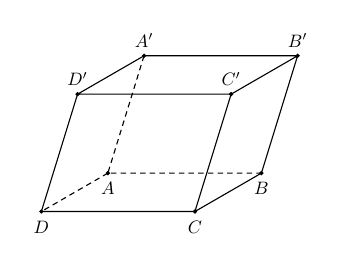
\begin{tikzpicture}[transform shape,scale=.65]
			\def\a{3}
			\path 
			(0:0) coordinate (A)++(-45:1) coordinate (H)
			(0:\a) coordinate (B)++(-150:\a/2) coordinate (C) ++ (180:\a) coordinate (D)
			(H)++(90:\a) coordinate (A')++(0:\a) coordinate (B')++(-150:\a/2) coordinate (C') ++ (180:\a) coordinate (D')
			;
			\draw[dash pattern=on 2pt off 1.5pt] (A')--(A)--(B) (A)--(D);
			\draw (D')--(A')--(B')--(C') (B)--(B') (C)--(B)
			(D')--(D)--(C)--(C')--cycle ;
			\foreach \x/\g in {A/-90,B/-90,C/-90,D/-90,A'/90,B'/90,C'/90,D'/90} \draw[fill=black] (\x) circle (.03)
			+(\g:.3) node{$\x$};
		\end{tikzpicture}	
	}
	\dapso{$h=4a$. }
	\loigiai{
		Ta có $S_{ABCD}=2.S_{ABC}=AB.BC.\sin\widehat{ABC}=\dfrac{a^2\sqrt{2}}{2}$.\\
		Vậy khoảng cách giữa hai đáy $ABCD$ và $A'B'C'D'$ là $h=\dfrac{V_{ABCD.A'B'C'D'}}{S_{ABCD}}=\dfrac{2\sqrt{2}a^3}{\dfrac{a^2\sqrt{2}}{2}}=4a$.
	}
\end{bt}
\begin{bt}%[DCHT Toán 11 - KNTT -Vũ Hồng Toàn]%[1K7KQ-3]
	Cho một khối lập phương biết rằng tăng độ dài cạnh của khối lập phương thêm $2~\rm{cm}$ thì thể tích của nó tăng thêm $152~\rm{cm^3}$. Tìm độ dài cạnh của khối lập phương đã cho.	
	\dapso{$a=4~\rm{cm}$.}
	\loigiai{
		Gọi $a~\rm{cm}$ là độ dài cạnh của khối lập phương, với $a>0$.\\
		Khi đó thể tích của nó là $V=a^3~\rm{cm^3}$.\\ 
		Sau khi tăng thêm $2~\rm{cm}$, thì thể tích mới là $V'=(a+2)^3~\rm{cm^3}$.\\
		Từ giả thiết, ta có
		\allowdisplaybreaks
		\begin{eqnarray*}
			&&V'-V=152\\
			&\Leftrightarrow&(a+2)^3-a^3=152\\
			&\Leftrightarrow&6a^2+12a-144=0\\
			&\Leftrightarrow&\hoac{&a=-6&\text{ (loại)}\\ &a=4&\text{ (nhận)}.}
		\end{eqnarray*}
	}
\end{bt}
\begin{bt}%[DCHT Toán 11 - KNTT -Vũ Hồng Toàn]%[1K7GQ-3]
	\immini{
		Cho hình chóp $S.ABC$ có đáy là tam giác vuông tại $A$, $\widehat{ABC}=30^\circ$; $SBC$ là tam giác đều và nằm trên mặt phẳng vuông góc với đáy. Biết thể tích của khối chóp $S.ABC$ là $\dfrac{a^3}{4}$. Tính khoảng cách từ $C$ đến mặt phẳng $(SAB)$.	
	}
	{
		\begin{tikzpicture}[transform shape,scale=.65]
			\def\a{4.5}
			\def\h{3.5}
			\path 
			(0:0) coordinate (B)++(0:\a) coordinate (A)++(-130:\a/2) coordinate (C) 
			($(B)!.5!(C)$) coordinate (H)++(90:\h) coordinate (S);
			\draw[dash pattern=on 2pt off 1.5pt] (A)--(B);
			\draw (S)--(B)--(C)--cycle (C)--(A)--(S);
			\foreach \x/\g in {A/0,B/180,C/-90,S/90} \draw[fill=black] (\x) circle (.03)
			+(\g:.3) node{$\x$};
		\end{tikzpicture}	
	}
	\dapso{$\mathrm{d}(C,(SAB))=\dfrac{4a\sqrt{183}}{61}$.}
	\loigiai{
		\immini{
			Gọi $H$ là trung điểm của $BC$. Đặt $2x=BC$. Khi đó\\
			$\heva{&(SBC)\perp (ABC)\\&(SBC)\cap (ABC)=BC\\&SH\perp BC}	\Rightarrow SH\perp (ABC)$.\\
			$\triangle SBC$ đều nên $SH=x\sqrt{3}$.\\
			$\triangle ABC$ vuông tại $A$ nên $AB=BC\cdot \cos B=\dfrac{x\sqrt{3}}{2}$,~ $AC=\sqrt{BC^2-AB^2}=x$.
		}
		{
			\begin{tikzpicture}[transform shape,scale=.65]
				\def\a{4.5}
				\def\h{3.5}
				\path 
				(0:0) coordinate (B)++(0:\a) coordinate (A)++(-130:\a/2) coordinate (C) 
				($(B)!.5!(C)$) coordinate (H)++(90:\h) coordinate (S);
				\draw[dash pattern=on 2pt off 1.5pt] (A)--(B);
				\draw (S)--(B)--(C)--cycle (C)--(A)--(S)--(H)
				pic[draw, angle radius=2.5mm]{right angle=B--H--S}
				pic[draw, angle radius=2.5mm]{right angle=B--A--C}
				;
				\foreach \x/\g in {A/0,B/180,C/-90,H/220,S/90} \draw[fill=black] (\x) circle (.03)
				+(\g:.3) node{$\x$};
			\end{tikzpicture}		
		}
		\noindent
		$S_{ABC}=\dfrac{1}{2}AB.AC=\dfrac{x^2\sqrt{3}}{4}$.\\
		Mà $V_{S.ABC}=\dfrac{1}{3}S_{ABC}\cdot SH\Leftrightarrow \dfrac{a^3}{16}= \dfrac{1}{3}\cdot \dfrac{x^2\sqrt{3}}{4}\cdot x\sqrt{3} \Leftrightarrow x=a$.\\
		$\triangle SAH$ vuông tại $H$ có $AH=\dfrac{BC}{2}=x$ và $SA=\sqrt{SH^2+AH^2}=2a\Rightarrow \triangle SAB$ cân tại $S$,\\ $S_{SAB}=\dfrac{a^2\sqrt{183}}{16}$ (công thức Heron).\\
		Khi đó $V=V_{C.SAB}	=\dfrac{1}{3}\cdot S_{SAB}\cdot \mathrm{d}(C,(SAB))\Rightarrow \mathrm{d}(C,(SAB))=\dfrac{3V}{S_{SAB}}=\dfrac{4a\sqrt{183}}{61}$.
	}
\end{bt}

\centerline{\fcolorbox{teal}{yellow!50}{\bf {CÂU HỎI TRẮC NGHIỆM}}}
% (10 câu theo theo tỉ lệ 4:3:2:1)
\Opensolutionfile{ans}[ans/ans-1K7-27-4]

\begin{ex}%[DCHT Toán 11 - KNTT -Vũ Hồng Toàn]%[1K7YQ-3]
	Nếu có một khối chóp có thể tích và diện tích mặt đáy lần lượt bằng $a^3$ và $a^2$ thì chiều cao của nó bằng
	\choice
	{$a$}
	{\True $3a$}
	{$2a$}
	{$\dfrac{a}{3}$}	
	\loigiai
	{
		Ta có $V=\dfrac{1}{3}S.h\Rightarrow h=\dfrac{3V}{S}=3a$.
	}
\end{ex}
%Cau2
\begin{ex}%[DCHT Toán 11 - KNTT -Vũ Hồng Toàn]%[1K7YQ-3]
	\immini{
		Cho khối lập phương $ABCD.A'B'C'D'$ có thể tích bằng $8a^3$. Tính độ dài đoạn thẳng $A'C$.
		\choice[2]
		{\True $2a\sqrt{3}$}
		{$a\sqrt{3}$}
		{$2a\sqrt{2}$}
		{$a\sqrt{2}$}	
	}
	{
		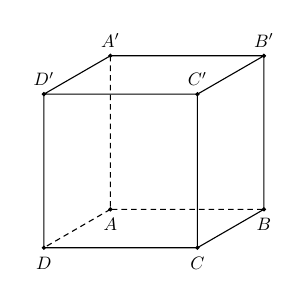
\begin{tikzpicture}[transform shape,scale=.65]
			\def\a{3}
			\path 
			(0:0) coordinate (A)
			(0:\a) coordinate (B)++(-150:\a/2) coordinate (C) ++ (180:\a) coordinate (D)
			(90:\a) coordinate (A')++(0:\a) coordinate (B')++(-150:\a/2) coordinate (C') ++ (180:\a) coordinate (D')
			;
			\draw[dash pattern=on 2pt off 1.5pt] (A')--(A)--(B) (A)--(D);
			\draw (D')--(A')--(B')--(C') (B)--(B') (C)--(B)
			(D')--(D)--(C)--(C')--cycle ;
			\foreach \x/\g in {A/-90,B/-90,C/-90,D/-90,A'/90,B'/90,C'/90,D'/90} \draw[fill=black] (\x) circle (.03)
			+(\g:.3) node{$\x$};
		\end{tikzpicture}		
	}
	\loigiai
	{
		Đặt $AB=x,x>0$.\\ Khi đó $V=x^3\Leftrightarrow x^3=8a^3=(2a)^3\Leftrightarrow x=2a$.\\
		$\triangle A'AC$ vuông tại $A$ có $A'C=\sqrt{A'A^2+AB^2+AD^2}=\sqrt{x^2+x^2+x^2}=x\sqrt{3}=2a\sqrt{3}$.
	}
\end{ex}
%Cau3
\begin{ex}%[DCHT Toán 11 - KNTT -Vũ Hồng Toàn]%[1K7YQ-3]
	\immini{
		Cho khối lăng trụ $(\mathscr{H})$ có thể tích là $4a^3$, đáy là tam giác vuông cân có độ dài cạnh huyền bằng $a\sqrt{2}$. Chiều cao $h$ của khối lăng trụ $(\mathscr{H})$ bằng
		\choice
		{$4a$}
		{\True $8a$}
		{$6a$}
		{$2a$}	
	}
	{
		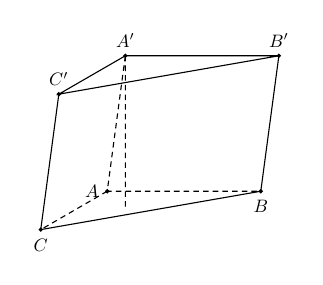
\begin{tikzpicture}[transform shape,scale=.65]
			\def\a{3}
			\path 
			(0:0) coordinate (A)++(-45:.5) coordinate (H)
			(0:\a) coordinate (B) (A)++(-150:\a/2) coordinate (C)
			(H)++(90:\a) coordinate (A')++(0:\a) coordinate (B') (A')++(-150:\a/2) coordinate (C') ;
			\draw[dash pattern=on 2pt off 1.5pt] (A')--(A)--(B) (A)--(C) (A')--(H);
			\draw (A')--(B')--(C')--cycle (B')--(B)--(C)--(C');
			\foreach \x/\g in {A/180,B/-90,C/-90,A'/90,B'/90,C'/90} \draw[fill=black] (\x) circle (.03)
			+(\g:.3) node{$\x$};
		\end{tikzpicture}	
	}
	\loigiai
	{
		$\triangle ABC$ vuông cân tại $A$ nên nếu gọi $H$ là trung điểm của $BC$ thì $AH\perp BC$ và $AH=\dfrac{BC}{2}=\dfrac{a\sqrt{2}}{2}$.\\
		$S=S_{ABC}=\dfrac{1}{2}AH.BC=\dfrac{1}{2}\cdot \dfrac{a\sqrt{2}}{2}\cdot a\sqrt{2}=\dfrac{a^2}{2}$.\\
		$V=S.h\Rightarrow h=\dfrac{V}{S}=\dfrac{4a^3}{\dfrac{a^2}{2}}=8a$.
	}
\end{ex}
%Cau4
\begin{ex}%[DCHT Toán 11 - KNTT -Vũ Hồng Toàn]%[1K7BQ-3]
	\immini{
		Cho khối chóp $S.ABCD$ có thể tích bằng $2a^3$ và đáy $ABCD$ là hình bình hành. Biết diện tích tam giác $SAB$  bằng $a^2$ Tính khoảng cách giữa hai đường thẳng $SB$ và $CD$.
		\choice[2]
		{$\dfrac{a\sqrt{2}}{2}$}
		{$\dfrac{3a}{2}$}
		{\True $3a$}
		{$a$}	
	}
	{
		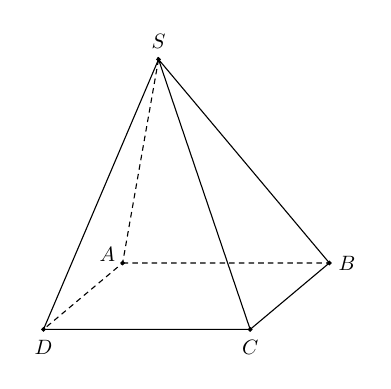
\begin{tikzpicture}[transform shape,scale=.75]
			\def\a{3.5}
			\path 
			(0:0) coordinate (A)++(0:\a) coordinate (B)++(-140:\a/2) coordinate (C) ++ (180:\a) coordinate (D) (80:\a) coordinate (S);
			\draw[dash pattern=on 2pt off 1.5pt] (S)--(A)--(D) (A)--(B);
			\draw (S)--(B)--(C)--cycle (C)--(D)--(S);
			\foreach \x/\g in {A/150,B/0,C/-90,D/-90,S/90} \draw[fill=black] (\x) circle (.03)
			+(\g:.3) node{$\x$};
		\end{tikzpicture}		
	}
	
	\loigiai
	{
		Ta có $AB\parallel CD\Rightarrow \mathrm{d}(SB,CD)=\mathrm{d}(CD,(SAB))=\mathrm{d}(C,(SAB))=\dfrac{3V_{S.ABC}}{S_{SAB}}=\dfrac{3\cdot \dfrac{1}{2}\cdot 2a^3}{a^2}=3a$.
	}
\end{ex}
%Cau5
\begin{ex}%[DCHT Toán 11 - KNTT -Vũ Hồng Toàn]%[1K7BQ-3]
	\immini{
		Gọi $V$  là thể tích của khối lập phương $ABCD.A'B'C'D'$, $V_1$  là thể tích khối tứ diện $A'ABC$. Hệ thức nào sau đây là đúng?
		\choice[2]
		{$V=4V_1$}
		{$V=3V_1$}
		{\True $V=6V_1$}
		{$V=8V_1$}		
	}
	{
		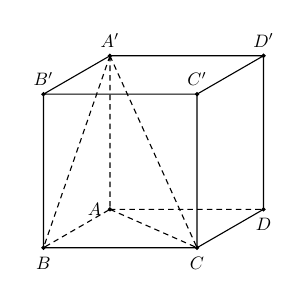
\begin{tikzpicture}[transform shape,scale=.65]
			\def\a{3}
			\path 
			(0:0) coordinate (A)
			(0:\a) coordinate (D)++(-150:\a/2) coordinate (C) ++ (180:\a) coordinate (B)
			(90:\a) coordinate (A')++(0:\a) coordinate (D')++(-150:\a/2) coordinate (C') ++ (180:\a) coordinate (B')
			;
			\draw[dash pattern=on 2pt off 1.5pt] (A')--(A)--(B) (A)--(D) (A')--(C)--(A) (A')--(B);
			\draw (D')--(A')--(B')--(C') (B)--(B') (C)--(B)
			(D')--(D)--(C)--(C')--cycle ;
			\foreach \x/\g in {A/180,B/-90,C/-90,D/-90,A'/90,B'/90,C'/90,D'/90} \draw[fill=black] (\x) circle (.03)
			+(\g:.3) node{$\x$};
		\end{tikzpicture}	
	}
	\loigiai
	{
		Giả sử cạnh của hình lập phương là  $a$, ta có $V=a^3$  và $V_1=\dfrac{1}{3}A'A\cdot S_{ABC}=\dfrac{1}{6}a^3$ suy ra $V=6V_1$.
	}
\end{ex}
%Cau6
\begin{ex}%[DCHT Toán 11 - KNTT -Vũ Hồng Toàn]%[1K5BG-2]
	\immini{
		Cho khối lăng trụ $ABC.A'B'C'$  có thể tích bằng $V$. Tính thể tích khối đa diện $B'C'ABC$ .
		\choice[2]
		{$\dfrac{3V}{4}$}
		{$\dfrac{V}{4}$}
		{$\dfrac{V}{2}$}
		{\True $\dfrac{2V}{3}$}	
	}
	{
		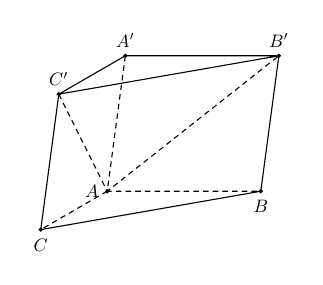
\begin{tikzpicture}[transform shape,scale=.65]
			\def\a{3}
			\path 
			(0:0) coordinate (A)++(-45:.5) coordinate (H)
			(0:\a) coordinate (B) (A)++(-150:\a/2) coordinate (C)
			(H)++(90:\a) coordinate (A')++(0:\a) coordinate (B') (A')++(-150:\a/2) coordinate (C') ;
			\draw[dash pattern=on 2pt off 1.5pt] (A')--(A)--(B) (A)--(C) (C')--(A)--(B');
			\draw (A')--(B')--(C')--cycle (B')--(B)--(C)--(C');
			\foreach \x/\g in {A/180,B/-90,C/-90,A'/90,B'/90,C'/90} \draw[fill=black] (\x) circle (.03)
			+(\g:.3) node{$\x$};
		\end{tikzpicture}	
	} 
	\loigiai
	{
		Gọi $h$ là chiều cao của khối lăng trụ $ABC.A'B'C'$.\\
		Ta có $V_{A.A'B'C'}=\dfrac{1}{3}S_{A'B'C'}\cdot h=\dfrac{1}{3}S_{ABC}\cdot h=\dfrac{V}{3}$.\\
		Mà $V=V_{A.A'B'C'}+V_{B'C'ABC}$.\\
		Vậy $V_{B'C'ABC}=V-V_{A.A'B'C'}=\dfrac{2V}{3}$.
	}
\end{ex}
%Cau7
\begin{ex}%[DCHT Toán 11 - KNTT -Vũ Hồng Toàn]%[1K7BQ-3]
	\immini{
		Hình hộp đứng $ABCD.A'B'C'D'$  có đáy là một hình thoi có góc nhọn bằng $\alpha$ , cạnh $a$. Diện tích xung quanh của hình hộp đó bằng $S$. Tính thể tích của khối hộp $ABCD.A'B'C'D'$.
		\choice[2]
		{$\dfrac{1}{2}a\cdot S\cdot \sin\alpha$}
		{$\dfrac{1}{6}a\cdot S\cdot \sin\alpha$}
		{$\dfrac{1}{8}a\cdot S\cdot \sin\alpha$}
		{\True $\dfrac{1}{4}a\cdot S\cdot \sin\alpha$}	
	}
	{
		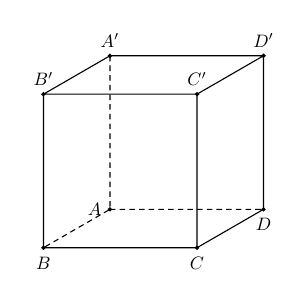
\begin{tikzpicture}[transform shape,scale=.65]
			\def\a{3}
			\path 
			(0:0) coordinate (A)
			(0:\a) coordinate (D)++(-150:\a/2) coordinate (C) ++ (180:\a) coordinate (B)
			(90:\a) coordinate (A')++(0:\a) coordinate (D')++(-150:\a/2) coordinate (C') ++ (180:\a) coordinate (B')
			;
			\draw[dash pattern=on 2pt off 1.5pt] (A')--(A)--(B) (A)--(D);
			\draw (D')--(A')--(B')--(C') (B)--(B') (C)--(B)
			(D')--(D)--(C)--(C')--cycle ;
			\foreach \x/\g in {A/180,B/-90,C/-90,D/-90,A'/90,B'/90,C'/90,D'/90} \draw[fill=black] (\x) circle (.03)
			+(\g:.3) node{$\x$};
		\end{tikzpicture}	
	} 
	\loigiai
	{
		Ta có $S=4AB.A'A\Rightarrow A'A=\dfrac{S}{4a}$.\\
		Mà $S_{ABCD}=2 S_{ABC}=2\cdot \dfrac{1}{2}AB\cdot BC\cdot \sin\alpha=a^2\sin\alpha$.\\
		Vậy $V=S_{ABCD}.A'A=a^2\sin\alpha\cdot \dfrac{S}{4a}=\dfrac{1}{4}a\cdot S\cdot \sin\alpha$.
	}
\end{ex}
%Cau8
\begin{ex}%[DCHT Toán 11 - KNTT -Vũ Hồng Toàn]%[1K7KQ-3]
	\immini{
		Cho hình lăng trụ tam giác $ABC.A'B'C'$  có đáy là tam giác đều cạnh $\sqrt{3}$ . Gọi  $I$ là trung điểm của cạnh $B'C'$. Biết thể tích lăng trụ là  $V=6$, khoảng cách từ điểm $I$  đến mặt phẳng $ABC$  bằng
		\choice[2]
		{$8\sqrt{3}$}
		{$4\sqrt{3}$}
		{\True $\dfrac{8\sqrt{3}}{3}$}
		{$\dfrac{4\sqrt{3}}{3}$}	
	}
	{
		\begin{tikzpicture}[transform shape,scale=.85]
			\def\a{3}
			\path 
			(0:0) coordinate (A)++(-45:.5) coordinate (H)
			(0:\a) coordinate (B) (A)++(-40:\a/2) coordinate (C)
			(H)++(90:\a) coordinate (A')++(0:\a) coordinate (B') (A')++(-40:\a/2) coordinate (C') ($ (B')!.5!(C') $) coordinate (I);
			\draw[dash pattern=on 2pt off 1.5pt] (A)--(B);
			\draw (A')--(B')--(C')--cycle (B')--(B)--(C)--(C') (I)--(A')--(A)--(C) ;
			\foreach \x/\g in {A/180,B/-90,C/-90,A'/90,B'/90,C'/180,I/-30} \draw[fill=black] (\x) circle (.03)
			+(\g:.3) node{$\x$};
		\end{tikzpicture}	
	}
	
	\loigiai
	{
		Gọi $h$ là chiều cao của khối lăng trụ $ABC.A'B'C'$.\\
		Ta có $h=\mathrm{d}(I,(ABC))$ và $S_{ABC}=\dfrac{3\sqrt{3}}{4}$.\\
		Mà $V=h.S_{ABC}\Rightarrow h=\dfrac{V}{S_{ABC}}=\dfrac{6}{\dfrac{3\sqrt{3}}{4}}=\dfrac{8\sqrt{3}}{3}$.
	}
\end{ex}
%Cau9
\begin{ex}%[DCHT Toán 11 - KNTT -Vũ Hồng Toàn]%[1K7KQ-3]
	\immini{
		Cho khối chóp $S.ABCD$ có đáy $ABCD$  là hình vuông tâm $O$, cạnh bên $SA$ vuông góc với đáy và  $SA=a\sqrt{3}$. Biết diện tích tam giác $SAB$  là  $\dfrac{a^2\sqrt{3}}{2}$, khoảng cách từ điểm $B$ đến mặt phẳng $(SAC)$  là
		\choice[2]
		{\True $\dfrac{a\sqrt{2}}{2}$}
		{$\dfrac{a\sqrt{10}}{3}$}
		{$\dfrac{a\sqrt{10}}{5}$}
		{$\dfrac{a\sqrt{2}}{3}$}	
	}
	{
		\begin{tikzpicture}[transform shape,scale=.75]
			\def\a{3.5}
			\path 
			(0:0) coordinate (A)++(0:\a) coordinate (B)++(-140:\a/2) coordinate (C) ++ (180:\a) coordinate (D) (90:\a) coordinate (S) ($(A)!.5!(C)$) coordinate (O);
			\draw[dash pattern=on 2pt off 1.5pt] (S)--(A)--(D)--(B) (A)--(B) (A)--(C);
			\draw (S)--(B)--(C)--cycle (C)--(D)--(S);
			\foreach \x/\g in {A/150,B/0,C/-90,D/-90,S/90,O/-90} \draw[fill=black] (\x) circle (.03)
			+(\g:.3) node{$\x$};
		\end{tikzpicture}		
	}
	\loigiai
	{
		Tam giác $SAB$ vuông tại $A$ nên $S_{SAB}=\dfrac{1}{2}SA\cdot AB\Rightarrow AB= \dfrac{2S_{SAB}}{SA}=\dfrac{2\cdot \dfrac{a^2\sqrt{3}}{2}}{a\sqrt{3}}=a$.\\
		Mà $\heva{&BO\perp AC\\ & BO\perp SA}\Rightarrow BO\perp (SAC)$.\\
		Vậy $\mathrm{d}(B,(SAC))=BO=\dfrac{AC}{2}=\dfrac{a\sqrt{2}}{2}$.
	}
\end{ex}
%Cau10
\begin{ex}%[DCHT Toán 11 - KNTT -Vũ Hồng Toàn]%[1K7GQ-3]
	\immini{
		Cho hình chóp $S.ABC$  có đáy $ABC$ là tam giác vuông cân tại $A$, cạnh  $BC=2a\sqrt{3}$. Tam giác  $SBC$ cân tại $S$  và nằm trong mặt phẳng vuông góc với mặt phẳng đáy. Biết thể tích của khối chóp bằng  $a^3$, tính góc giữa $SA$  và mặt phẳng  $(SBC)$.
		\choice[2]
		{$30^\circ$}
		{\True $60^\circ$}
		{$45^\circ$}
		{$90^\circ$}
	}
	{
		\begin{tikzpicture}[transform shape,scale=.85]
			\def\a{4.5}
			\def\h{3.5}
			\path 
			(0:0) coordinate (B)++(0:\a) coordinate (A)++(-130:\a/2) coordinate (C) 
			($(B)!.5!(C)$) coordinate (H)++(90:\h) coordinate (S);
			\draw[dash pattern=on 2pt off 1.5pt] (A)--(B);
			\draw (S)--(B)--(C)--cycle (C)--(A)--(S)--(H)
			pic[draw, angle radius=2.5mm]{right angle=B--H--S}
			pic[draw, angle radius=2.5mm]{right angle=B--A--C}
			;
			\foreach \x/\g in {A/0,B/180,C/-90,H/220,S/90} \draw[fill=black] (\x) circle (.03)
			+(\g:.3) node{$\x$};
		\end{tikzpicture}		
	}
	\loigiai
	{
		Gọi $H$ là trung điểm của $BC$. Khi đó\\
		$\heva{&(SBC)\perp (ABC)\\ & (SBC)\cap (ABC)=BC\\ &AH\perp BC}\Rightarrow AH\perp (ABC)$.\\
		Mà $ABC$ là tam giác vuông cân tại $A$ nên $AH\perp BC\Rightarrow AH\perp (SBC)$.\\
		Suy ra hình chiếu vuông góc của $SA$ lên $(SBC)$ là $SH$ hay $\widehat{(SA,(SBC))}=\widehat{(SA,SH)}$.\\
		Mặt khác $ABC$ là tam giác vuông cân tại $A$ nên $AB=\dfrac{BC}{\sqrt{2}}=a\sqrt{6}$ và $S_{ABC}=\dfrac{AB^2}{2}=3a^2$.\\
		Đường cao $SH=\dfrac{3V_{S.ABC}}{S_{ABC}}=a$.\\
		Do đó $\tan\widehat{ASH}=\dfrac{a\sqrt{3}}{a}=\sqrt{3}$.\\
		Vậy $\widehat{(SA,(SBC))}=\widehat{(SA,SH)}=60^\circ$.
	}
\end{ex}

\Closesolutionfile{ans}
\begin{indapan}{10}
	{ans/ans-1K7-27-4}
\end{indapan}


